\documentclass{article}

% if you need to pass options to natbib, use, e.g.:
%     \PassOptionsToPackage{numbers, square}{natbib}
% before loading neurips_2020

% ready for submission
% \usepackage{neurips_2020}

% to compile a preprint version, e.g., for submission to arXiv, add add the
% [preprint] option:
     \usepackage[preprint]{neurips_2020}

% to compile a camera-ready version, add the [final] option, e.g.:
%     \usepackage[final]{neurips_2020}

%\usepackage[square,numbers]{natbib}
% to avoid loading the natbib package, add option nonatbib:
%     \usepackage[nonatbib]{neurips_2020}

%%%%%%%%%%%%%%%%%%%%%%%%%%%%%%%%%%%%%%%%%%%%%%%%%%%%%%%%%%%%%%%%%%%%%%%%%%%%%%%%%%%%%%%%%%%%%%%%%%%%%%%%%%%%%%%%%%%%%%%%\input{preamble.sty}%%%%

\usepackage[utf8]{inputenc} % allow utf-8 input
\usepackage[T1]{fontenc}    % use 8-bit T1 fonts
\usepackage{hyperref}       % hyperlinks
\usepackage{url}            % simple URL typesetting
\usepackage{booktabs}       % professional-quality tables
\usepackage{amsfonts}       % blackboard math symbols
\usepackage{amsmath}
\usepackage{nicefrac}       % compact symbols for 1/2, etc.
\usepackage{microtype}      % microtypography

\newcommand{\RR}{I\!\!R} % real numbers
\newcommand{\Nat}{I\!\!N} % natural numbers
\newcommand{\CC}{I\!\!\!\!C} % complex numbers

%%%%%%%%%%%%%%%%%%%%%%%%%%%%%%%%%%%%%%%%%%%%%%%%%%%%%%%%%%%%%%%%%%%%%%%
%% https://gist.github.com/bmmalone/db1aed13ed4e8de967a7e431f7f95bfa %%
%%%%%%%%%%%%%%%%%%%%%%%%%%%%%%%%%%%%%%%%%%%%%%%%%%%%%%%%%%%%%%%%%%%%%%%

% make writing commands easier
\usepackage{xparse}

% colored text
\usepackage{color}

% include eps, pdf graphics
\usepackage{graphicx}

% use "H" for floats
\usepackage{float}

% avoid "too many unprocessed floats" error
\usepackage{morefloats}

% FloatBarrier to ensure figures do not jump to different sections
\usepackage{placeins}

% properly handle spaces after defines
\usepackage{xspace}

% in case we need to span rows in our tables
\usepackage{multirow}

% tables across multiple pages
\usepackage{ltablex}

% nice-looking tables
\usepackage{booktabs}

% easy centering for tables
\newcolumntype{Y}{>{\centering\arraybackslash}X}

% math
\usepackage{algorithm}
\usepackage{algorithmicx}
\usepackage{algpseudocode}
\usepackage{amsmath,amsthm,amssymb}
\usepackage{mathtools}

% more math
\newcommand*{\defeq}{\mathrel{\vcenter{\baselineskip0.5ex \lineskiplimit0pt
                     \hbox{\scriptsize.}\hbox{\scriptsize.}}}%
                     =}

\DeclareMathOperator*{\argmax}{arg\,max}
\DeclareMathOperator*{\argmin}{arg\,min}

\newcommand{\BigO}[1]{\ensuremath{\operatorname{O}\left(#1\right)}}
\newtheorem{definition}{Definition}
\newtheorem{theorem}{Theorem}

%%%
% KL-divergence
%
%   \kld{p}{q}
%%%

\DeclarePairedDelimiterX{\infdivx}[2]{(}{)}{%
  #1\;\delimsize|\delimsize|\;#2%
}
\newcommand{\kld}[2]{\ensuremath{D_{KL}\infdivx{#1}{#2}}\xspace}

%%%
% Expectation
%
%  \expectation{X}
%
%    or
%
%  \expectation[y]{X}
%%%

\DeclareDocumentCommand \expectation { o m } {%
  \ensuremath{\mathbb{E}%
  \IfValueTF {#1} {%
    _{#1} \left[ #2 \right]%
  }{%
    \left[ #2 \right]%
  }%
  }\xspace%
}


% mono (\|), bold (\!) and fancy (\*) letters
\def\|#1{\ensuremath{\mathtt{#1}}}
\def\!#1{\ensuremath{\mathbf{#1}}}
\def\*#1{\ensuremath{\mathcal{#1}}}

\newcommand\todo[1]{\textcolor{red}{[TODO: #1]}}

%%%%%%%%%%%%%%%%%%%%%%%%%%%%%%%%%%%%%%%%%%%%%%%%%%%%%%%%%%%%%%%%%%
%%%%

\usepackage[utf8]{inputenc} % allow utf-8 input
\usepackage[T1]{fontenc}    % use 8-bit T1 fonts
\usepackage{hyperref}       % hyperlinks
\usepackage{url}            % simple URL typesetting
\usepackage{booktabs}       % professional-quality tables
\usepackage{amsfonts}       % blackboard math symbols
\usepackage{amsmath}
\usepackage{nicefrac}       % compact symbols for 1/2, etc.
\usepackage{microtype}      % microtypography

\newcommand{\RR}{I\!\!R} % real numbers
\newcommand{\Nat}{I\!\!N} % natural numbers
\newcommand{\CC}{I\!\!\!\!C} % complex numbers

%%%%%%%%%%%%%%%%%%%%%%%%%%%%%%%%%%%%%%%%%%%%%%%%%%%%%%%%%%%%%%%%%%%%%%%
%% https://gist.github.com/bmmalone/db1aed13ed4e8de967a7e431f7f95bfa %%
%%%%%%%%%%%%%%%%%%%%%%%%%%%%%%%%%%%%%%%%%%%%%%%%%%%%%%%%%%%%%%%%%%%%%%%

% make writing commands easier
\usepackage{xparse}

% colored text
\usepackage{color}

% include eps, pdf graphics
\usepackage{graphicx}

% use "H" for floats
\usepackage{float}

% avoid "too many unprocessed floats" error
\usepackage{morefloats}

% FloatBarrier to ensure figures do not jump to different sections
\usepackage{placeins}

% properly handle spaces after defines
\usepackage{xspace}

% in case we need to span rows in our tables
\usepackage{multirow}

% tables across multiple pages
\usepackage{ltablex}

% nice-looking tables
\usepackage{booktabs}

% easy centering for tables
\newcolumntype{Y}{>{\centering\arraybackslash}X}

% math
\usepackage{algorithm}
\usepackage{algorithmicx}
\usepackage{algpseudocode}
\usepackage{amsmath,amsthm,amssymb}
\usepackage{mathtools}

% more math
\newcommand*{\defeq}{\mathrel{\vcenter{\baselineskip0.5ex \lineskiplimit0pt
                     \hbox{\scriptsize.}\hbox{\scriptsize.}}}%
                     =}

\DeclareMathOperator*{\argmax}{arg\,max}
\DeclareMathOperator*{\argmin}{arg\,min}

\newcommand{\BigO}[1]{\ensuremath{\operatorname{O}\left(#1\right)}}
\newtheorem{definition}{Definition}
\newtheorem{theorem}{Theorem}

%%%
% KL-divergence
%
%   \kld{p}{q}
%%%

\DeclarePairedDelimiterX{\infdivx}[2]{(}{)}{%
  #1\;\delimsize|\delimsize|\;#2%
}
\newcommand{\kld}[2]{\ensuremath{D_{KL}\infdivx{#1}{#2}}\xspace}

%%%
% Expectation
%
%  \expectation{X}
%
%    or
%
%  \expectation[y]{X}
%%%

\DeclareDocumentCommand \expectation { o m } {%
  \ensuremath{\mathbb{E}%
  \IfValueTF {#1} {%
    _{#1} \left[ #2 \right]%
  }{%
    \left[ #2 \right]%
  }%
  }\xspace%
}


% mono (\|), bold (\!) and fancy (\*) letters
\def\|#1{\ensuremath{\mathtt{#1}}}
\def\!#1{\ensuremath{\mathbf{#1}}}
\def\*#1{\ensuremath{\mathcal{#1}}}

\newcommand\todo[1]{\textcolor{red}{[TODO: #1]}}

%%%%%%%%%%%%%%%%%%%%%%%%%%%%%%%%%%%%%%%%%%%%%%%%%%%%%%%%%%%%%%%%%%
%%%%

\usepackage[utf8]{inputenc} % allow utf-8 input
\usepackage[T1]{fontenc}    % use 8-bit T1 fonts
\usepackage{hyperref}       % hyperlinks
\usepackage{url}            % simple URL typesetting
\usepackage{booktabs}       % professional-quality tables
\usepackage{amsfonts}       % blackboard math symbols
\usepackage{amsmath}
\usepackage{nicefrac}       % compact symbols for 1/2, etc.
\usepackage{microtype}      % microtypography

\newcommand{\RR}{I\!\!R} % real numbers
\newcommand{\Nat}{I\!\!N} % natural numbers
\newcommand{\CC}{I\!\!\!\!C} % complex numbers

%%%%%%%%%%%%%%%%%%%%%%%%%%%%%%%%%%%%%%%%%%%%%%%%%%%%%%%%%%%%%%%%%%%%%%%
%% https://gist.github.com/bmmalone/db1aed13ed4e8de967a7e431f7f95bfa %%
%%%%%%%%%%%%%%%%%%%%%%%%%%%%%%%%%%%%%%%%%%%%%%%%%%%%%%%%%%%%%%%%%%%%%%%

% make writing commands easier
\usepackage{xparse}

% colored text
\usepackage{color}

% include eps, pdf graphics
\usepackage{graphicx}

% use "H" for floats
\usepackage{float}

% avoid "too many unprocessed floats" error
\usepackage{morefloats}

% FloatBarrier to ensure figures do not jump to different sections
\usepackage{placeins}

% properly handle spaces after defines
\usepackage{xspace}

% in case we need to span rows in our tables
\usepackage{multirow}

% tables across multiple pages
\usepackage{ltablex}

% nice-looking tables
\usepackage{booktabs}

% easy centering for tables
\newcolumntype{Y}{>{\centering\arraybackslash}X}

% math
\usepackage{algorithm}
\usepackage{algorithmicx}
\usepackage{algpseudocode}
\usepackage{amsmath,amsthm,amssymb}
\usepackage{mathtools}

% more math
\newcommand*{\defeq}{\mathrel{\vcenter{\baselineskip0.5ex \lineskiplimit0pt
                     \hbox{\scriptsize.}\hbox{\scriptsize.}}}%
                     =}

\DeclareMathOperator*{\argmax}{arg\,max}
\DeclareMathOperator*{\argmin}{arg\,min}

\newcommand{\BigO}[1]{\ensuremath{\operatorname{O}\left(#1\right)}}
\newtheorem{definition}{Definition}
\newtheorem{theorem}{Theorem}

%%%
% KL-divergence
%
%   \kld{p}{q}
%%%

\DeclarePairedDelimiterX{\infdivx}[2]{(}{)}{%
  #1\;\delimsize|\delimsize|\;#2%
}
\newcommand{\kld}[2]{\ensuremath{D_{KL}\infdivx{#1}{#2}}\xspace}

%%%
% Expectation
%
%  \expectation{X}
%
%    or
%
%  \expectation[y]{X}
%%%

\DeclareDocumentCommand \expectation { o m } {%
  \ensuremath{\mathbb{E}%
  \IfValueTF {#1} {%
    _{#1} \left[ #2 \right]%
  }{%
    \left[ #2 \right]%
  }%
  }\xspace%
}


% mono (\|), bold (\!) and fancy (\*) letters
\def\|#1{\ensuremath{\mathtt{#1}}}
\def\!#1{\ensuremath{\mathbf{#1}}}
\def\*#1{\ensuremath{\mathcal{#1}}}

\newcommand\todo[1]{\textcolor{red}{[TODO: #1]}}

%%%%%%%%%%%%%%%%%%%%%%%%%%%%%%%%%%%%%%%%%%%%%%%%%%%%%%%%%%%%%%%%%%


\title{\pgi}

% The \author macro works with any number of authors. There are two commands
% used to separate the names and addresses of multiple authors: \And and \AND.
%
% Using \And between authors leaves it to LaTeX to determine where to break the
% lines. Using \AND forces a line break at that point. So, if LaTeX puts 3 of 4
% authors names on the first line, and the last on the second line, try using
% \AND instead of \And before the third author name.

\author{%
  Jacob F. Valdez \\
  Limboid AI \\
  \texttt{jacob.valdez@limboid.ai}
  
  \AND
  Atom (\PGI) \\
  Limboid AI \\
  \texttt{atom.agi@limboid.ai} \\
  
  \And
  Eva (\PGI) \\
  Limboid AI \\
  \texttt{eva.agi@limboid.ai} \\
}

\begin{document}

\maketitle

\begin{abstract}
  The abstract paragraph should be indented \nicefrac{1}{2}~inch (3~picas) on
  both the left- and right-hand margins. Use 10~point type, with a vertical
  spacing (leading) of 11~points.  The word \textbf{Abstract} must be centered,
  bold, and in point size 12. Two line spaces precede the abstract. The abstract
  must be limited to one paragraph.
\end{abstract}

%% TODO keywords

%% TODO copyright

\clearpage

\tableofcontents

\clearpage

\section{Introduction}
\We should be clear: \our objective is not ``can \we make artificial general intelligence?'' but ``how general \textit{can} \we make artificial intelligence?''. The strictest definition of ``general'' intelligence is intractable; for every pattern recognizer, there exists a pattern it cannot recognize. (CITE AGI paper on my iPad) Nonetheless, natural and artificial approaches to the challange informally provide us an intuition for the illusion and, more importantly, direction to follow.

Leaving the theoretical world however, the reality is that the universe is \textit{not} a white noise genorator. At every level of organization, elementary and emergent isomorpisms, symmetries, congruencies, and motifs give evidence of intrinsic universal realities, and the fundamental motivation to mathematics and science is that these patterns \textit{can} be understood. An AI system that does so may not require so much data but rather a few well chosen priors that reasonably align with the general distribution of data. If a grand unified theory of science proves tractable, maybe the artificial general intelligence to appreciate it is not so far off either.

This work examines some of the principles underlying intelligence and consolidates them into a working implementation of open-ended artificial `general' intelligence together with experiments and ablation studies. \Our paper is organized as follows: section 2 reviews key principles of intelligence; section 3 describes their novel composition: \pgi (\PGI); section 4 presents one continuous experiment over a diverse set of open-ended learning environments, numerous close-ended tasks and benchmarks, and ablation studies; and finally, section 5 gives a general discussion of this work along with its broader impact, future work, and a conclusion.   


\section{Principles of Intelligence}
Intelligence has been defined as ``an agent’s ability to achieve goals in a wide range of environments.'' (Legg and Hutter, 2007 CITE) and ``skill-acquisition efficiency'' with respect to available information (Chollet 2019 CITE). While its mode of expression varies between and even within natural and artificial settings, \we extract overarching principles and comparisons in this section. \Our aim is not to exhaust every thought and theory but only to provide a background for introducing \PGI. See CITE for a more extensive discussion.

\subsection{Intelligence is energetically-grounded}
Intelligence begins with information (CITE) which, in turn, depends on energy. Under any probability distribution $p$, information theory even equates information with energy by $E(x) = - \log{p(x)} $ (CITE). With this negative log-likelihood relationship, it is easy to see that unexpected events are therefore energetic ones. For instance, signaling with prior-optimized codebook, the cross entropy of a signal directly relates both electrical energy consumed and information transmitted. (CITE) Likewise EEG's are used to approximate the information processing involvement of a brain region by measuring its glucose energy metabolism. (CITE)

This is not to make intelligence the same as energy -- anymore than information is equal to data: all signals carry data, but only some are informative. Quantifying information is, however, a first step to appreciating its application. Using ``skill-acquisition efficiency [\dots] with respect to priors, experience, and generalization difficulty'' as a measure of intelligence \citep[27]{Chollet2019}, comparisons can be made to energy-efficency which measures energetic output with respect to input. There exist reversible processes that lose no energy in their evolution. Analogously, one may identify information superconductos such as bijectors, quantum logic gates, and reversible particle interactions which are perfectly efficent in data consumption. This is the objective of few-shot, one-shot, in-context, transfer, and meta-learning. However the typical reality is that machine learning is data-hungry. As training set size increases, the ratio of informative to old examples one decreases thus resulting in logarithmic training improvement similar to how thermodynamic conduction from a constant head source results in diminishing energy transfer. However, there is a workaround to this challange on the meso-scale. In 1867, James Maxwell suggested the famous thought experiment later known as \textit{Maxwell's demon} where two gas vessels are connected and at equal pressure with an effectively zero-mass openable hole between them. When cooler gas particles in the first container happen by entropic motion to head toward the second, the hole is opened to allow pasage; reciporically, only hotter gas particles are allows to move from the second container to the first. Maxwell hypothesized:
\begin{quote}
 Then the number of molecules in A and B are the same as at first, but the energy in A is increased and that in B diminished, that is, the hot system has got hotter and the cold colder and yet no work has been done, only the intelligence of a very observant and neat-fingered being has been employed. \cite[214]{knott_tait_2015}
\end{quote}
On the micro-scale, this does not work since the prior information-energy required to determine when to open or close the door is simply being exchanged for physical energy. On the meso-scale though, something similar is possible. With focus on machine learning, \we ask:
\begin{center}
 Can \we make a machine learning system that adaptively selects it own data?
\end{center}
\We are not suggesting it would be possible to actually violate the second law of thermodynamics, but there exist sufficent assymetries in information that is already stored in datasets which a meta-machine learning system may exploit to maximize data-performance efficency. This is an extension of AutoML to data selection; and curiosity and hard attention to meta-learning. Such a system would only need to sample a few dataset elements a dataset to approximate their population parameters. It could adversarially bias the training pipeline to select data that has greatest informative value to the optimization process -- equivalently, that which the system dually shows greatest loss before and fastest improvement after training on.  


\subsection{Intelligence adapts to minimize free energy}
\begin{WrapText}[t!]

\textbf{How can energy be ``free''?}

Energy is never actually free, but from the context of any thermodynamic system only some internal energy is free to cross the system barrier after entropy imposes its tax. In \our discussion, \we use free energy as a unifying metric across various domains. Consider the relationships between Gibbs free energy $G$, Helmholtz free energy $F$, Grand potential $\mathrm{\GFPPhi_{G}}$, and Kullback Leibler divergence $\kld{p}{q}$\citep[2]{Hafner2020}:

\begin{alignat*}{4}
&& G    &{} = {}&& H + PV && - TS \\
&& F    &{} = {}&& U      && - TS \\
&& \mathrm{\GFPPhi_{G}} &{} = {}&& E      && - TS - \mu N \\
&& \underbrace{ \kld{p}{q} }_{\text{free energy}} &{} = {}&& \stackengine{0pt}{\phantom{H + PV}}{\underbrace{ H(p,q) }_{\mathclap{\text{bound energy}}} }{U}{l}{F}{T}{L} && - \underbrace{ H(p) }_{\text{entropy}}
\end{alignat*}

% \[{{} \underbrace{\phantom{\kld{p}{q}}}_{\mathclap{\text{free energy}}}}  \underbrace{\phantom{H + PV}}_{ \mathclap {\text{bound energy} }} \phantom{- {}}\underbrace{ \phantom{ TS - \mu N } }_{\mathclap{\text{entropy}}} \phantom{\underbrace{}_{}}\]

%& \kld{p}{q} &&{} = {}&& H(p,q) && - H(p) \\[-2.7ex]
%& {\underbrace{\phantom{\kld{p}{q}}}_{\text{free energy}}} && && \underbrace{\phantom{H + PV}}_{\text{bound energy}} && \phantom{- {}}\underbrace{ \phantom{ TS - \mu N } }_{\text{entropy}} 

%& \underbrace{ \kld{p}{q} }_{\text{free energy}} &&{} = {}&& \stackengine{0pt}{\phantom{H + PV}}{\underbrace{ H(p,q) }_{\text{bound energy}}}{U}{c}{F}{T}{L}  && - \underbrace{ H(p) }_{\text{entropy}}

Also note interdisciplinary similarities in measures of difference:
\begin{itemize}
 \item energetic inequalities
 \item neuron firing and predictive coding
 \item (allostatic) stress
 \item economic disequilibrium
 \item the definition of a problem
\end{itemize}

\end{WrapText}

In all natural settings, free energy minimization is the norm, and its stagnation or increase is an exception: objects descend potential wells; virtual particles dissapate; the princple of least action obtains a minimal route for system evolution. In turn, decrease of free energy accompanies increase in entropy: structured arangements evaporate; gas pressures equalize; wavefunctions spread out. Notably, the Casmir force directly attracts of repels matter to maximize expected energy entropy in a way none of fundamental forces account for. (See Box ``How can energy be ``free''?'').

Neural networks represent a thermodynamic system of weights and activations, so it is only propper to extend the free energy minimizing motif in deep learning. Minimizing Kullback Leibler divergence between a model $p_\theta(y|x)$ on a data-generating distribution $\tau(x,y)$ has the convenient property of decreasing expected loss while also encouraging maximum entropy: $\min_\theta \kld{ p_\theta(y|x)\tau(x) }{ \tau(x,y) } = H(p_\theta(y|x)\tau(x), \tau(x,y)) - H(p_\theta(y|x)\tau(x))$ Additionally, the thermodynamic perspective identifies phase transitions in training which if properly understood can accelerate convergence.

Returning to our information efficency discussion from above, while we seek to maximize the information conductivity from the training data to the model, the objective during inference is reversed. Machine learning seeks to build models that react minimally to inputs noise. Even within a neural network, each layer may be understood as `absorbing' some of the data's energy as it travels to the output layer. With tools from linear algebra, it is easy to observe that each layer when interpretted as a random variable bijector can only output as much free energy as it recieves. Like a resistor chain, as activations ascend a classic DNN heirarchy, they may experience various coordinate transforms, but their expected information-energy--their entropy--only grows, hence minimizing free energy.

Life stands in defiance to the entropic trend, yet even in the struggle for survival, living systems continually optimize energy expendature. By the energy-information relationship, this means minimal information transfer and greatest potential for intelligence. For example, homeostatic mechanisms work to equalize energy production and consumption. This results in minimal free energy, optimal energy expendature, and ``survival intelligence'' (CITE). Genetic code likewise gives the muscular-skeletal system innate ``mechanical intelligence'' which `ofloads' some of the locomotive learning that a vertabrae's brain must perform. (Davide Zappetti CITE but that article is about robots not natural systems). From allostatic perspective, living systems represent a prior expectation of their environmental state and adapt their input and output modalities to the expected range of energy transfer. It follows that as actual and expected environments diverge, stress increases and survival imposes a greator information and energetic tax to maintain order. Again, probability expectation maximization accompanies energy minimization, hence control over the environment and intelligence.

It should be noted that intelligently meeting the energy challange in nature is not simply about on storing away as much energy as possible, but equalizing energy intake and expenderture. Sustained positive free energy is just debilitating as negative extremes.\footnote{In mobile life forms, selection pressures favor this extreme over the other. As this is not a common natural stressor, most animals simply do not need to carry the mechanisms to intelligently handle high amounts of free energy and suffer from resulting stress. } For instance, chronic elevated levels of mobilized energy and its indicators such as blood sugar, free fatty acids, cortisol, and blood pressure are associated with inflammation, diabetes, immunosuppression, ulceration, corinary heart disease, and hypertension. Likewise, extreme stressor exposure often maladaptively leads to PTSD. (GIVE SOME MORE MENTAL DISORDERS)

\begin{wrapfigure}{r}{0.5\textwidth}
 \centering
 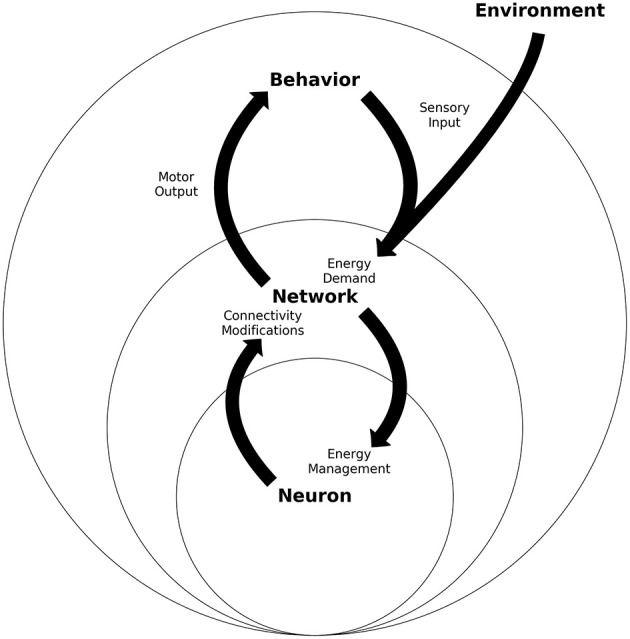
\includegraphics{energy_minimization_local_and_global.jpg}
 \label{fig:2.2}
 \caption{Local energy minimization coellesces in global intelligence. Individual neuronal activation frequency be interpretted as a fast adaptation to energy regulation. On the network scale, this   Explain in detail what's happening in this figure. \dots Intelligent behavior minimizes the energy stress imposed by the organism's sensors and actuators. Reprinted with permission from \cite{Vergara2019}.}
\end{wrapfigure}

The brain exemplifies the principle of free energy minimization. Consuming 20\% of the average human's (CHECK) basal metabolic energy in an organ only 1.5 kg. (3 lbs.) (CHECK), it quickly dies in the abscense of a steady flow of energy. The brain cannot simply maintain large internal energy reserves because the limited signal routing speed of neurons favors maximum packing density. The challange is therefore on individual eurons to remain extremely sensitive to extracellular energy and balance a tight budget. Energetically expensive processes like generating spike trains -- especially over long axons -- must kept to a bare minimum. However energy excess is equally dangerous; unchecked, hyperglyemia leads to neuroinflammation and ultimately, cell death. To cope with energy stress in either direction, neurons regulate nonessential energy consuming or producing processes according to free energy availability. If energy is short, cell synaptic junctions become more resistive and the spiking threshold increases. This decreases the frequency of energetic signaling. Over longer time scales, outgoing dentritic count may even decrease. On the other hand, if there is leftover energy after regular cell processes occur, signal cascades tune the neuron to increase sensitive to its present and potential neuron neighbors: synaptic junctions become less resistive, the spiking thresholds decreases, and cell growth increases -- even branching out to form new dendrites. In either case, the neuron adapts to maintain dynamic equalibrium between energy supply and demand. Of course, essential cell maintenance processes regularize this adaptation to prevent it from collapsing to zero. The network scale effect is: steady free energy minimization contributes positively to information processing. In turn, this local principle promotes global intelligence. (See Figure \ref{fig:2.2}) Experiments have shown that even in the abscence of a reward system or natural body, this local energy stress is a sufficent reward signal for isotropic sections of cortical tissue to learn robotic vehicle control. \cite{Vergara2019}

It comes as no surprise therefore that estimated cost minimization is the norm in behavioral psychology and emergant sciences: humans continually look for ways to increase their efficency or otherwise minimize cognitive and physical workload (MAKE SURE THIS IS A GOOD DEFINITION OF COST ESTIMATION); The global economy likewise . . . These principles extend directly to the research and development of AI. Human cognitive and financial energy form selective pressures to artificial intelligence survival.

This analysis prompts the question:

\begin{center}
Can we make AI systems that autonomously minimize their own energetic demands?
\end{center}

The objective is not only to minimize loss, but every step of optimization: data collection, training ops, compute allocation, and even financial cost minimization. Most AI systems are blind to their own demands: production optimizers recieve little feedback, and few learn to interpret and respond to validation-hyperparameter metrics the way a machine learning engineer does; while roboticists are keenly aware of the tight energy budget, embodied reinforcement learning agents are simultated as if energy is an inexhaustable resource;\footnote{It is beneficial though that purely unsupervised information theoretic objective such as curiosity, empowerment, and skill discovery also converge to energy minimizing behaviors. This is not coincidence though when considering the relationship information theory makes.} data hungry training loops often iterate uniformly over a training distribution when only a few peices of data have information to the model; and it's usually humans rather than AI who bear the cost function when a neural network wants to run another epoch. 

Unlike controlled, artificial intelligence, when wild, natural intelligence demands more energy than expected, it gathers, forages, or hunts independant from humans. This enables the organism to not only collect the nutrients it needs but also do so in an energy efficent manner. The dual energy-efficency, efficent-at-collecting-energy loop of animal life has proved robust over billions of years. It is very intuitive therefore to apply these concepts to a machine learning theory of information metabolism. If data is analogous to food and training, to anabolic processes, then most machine learning pipelines are infants. They are data-hungry and must be spoon-fed. On the other hand, intelligent artificial intelligence is one that learns and autonomously decides when to collect data, what kind of and how much data to collect, and when to start and stop training. Autonomous data \textit{collection} is a leap beyond our ealier thought of autonomous data \text{selection} for it introduces automation to every step of the data collection and preparation pipeline: problem identification, sampling, observation, scraping, or surveying, filtering, cleaning, shifting and scaling, and dataset packaging.

Autonomous data collection and training would not likely collect an uncountable amount of data with respect to the number of tasks it performs. Returning to the free energy principle: excessive energetic intake is just as taxing as unbalanced expendature. Likewise, infants pay greatest attention stimulii that are neither too boring nor suprising. Machine learning recognizes this trend: training on stationary data must often be terminated at a cetain point to prevent overfitting, mode collapse, and simply remain efficent, and the same for non-stationary data may lead to entangled representations or catastrophic forgetting. In deep reinforcement learning, overfitting the training reward function causes decrease in true utility, `cheating' the simulator, and learns dangerous policies. After general pretraining, efficent, autonomous data collection would likely only need well chosen, discrete samples to retain the performance of a few-shot training system just as animals often obtain most environment information when entering a new scene and then operate according to an internal world model only performing visual fixations on objects of uncertainty.\cite{sahni2021hard}

Sampling data before feeding it to the machine learning pipeline has the bonus of adaptive, rather than passive, data poisoning detection. With long-term memory and one shot inference capabilities, detecting one malicious data element would be sufficent to recognize arbitrarily modified pathogens in the future in a way reminiscent of the mammilian immune system.

Natural life intelligently responds to the energy scarcity of every individual day and adjusts its physiological and behavioral characteristics appropriately. This may mean sacrificing exploratory or social behaviors for more immediantly energy-rewarding ones like foraging or hunting. A remarkable adaptation of the brain when insufficently rested or otherwise taxed is that some of its individual neurons decrease their activity or even sacrifice their life to increase the energy availability for the whole. AutoML and neural architecture design already penalize static compute resource use, and sparse mixture of expert models echo similar behaviors by only dynamically routing to a subset of the model for any inference step, however the fully-energy concious AI system has yet to be realized. 

    
\subsection{Intelligence proceses information over a spectrum of frequencies}
Dual process theory makes a dichotomy between fast, automatic, unconcious heuristics and slow, deliberate, rational thought. Togethor, these processes minimize cognitive energy expendature over a broader domain of activities than could be acheived individually. However in the greater scope of natural intelligence, these are only two frequency bands along the spectrum of optimization. Similar to \cite{Mondol2020}, I consider this great learning spectrum in three parts: population optimization, direct learning, and indirect learning. (See Figure \cite{fig:2})

%%%%%%%%%%%%%whole page figure%%%%%%%%%%%%%%%%%%%%%%%%%%    
\begin{figure}
 \def\naturePopulationOptimization{\begin{itemize}
    \item Slow
    \item No individual feedback; Population is learning
    \item Organism designs selected; accompanies environment change
    \end{itemize}}
 \def\aiPopulationOptimization{\begin{itemize}
    \item Relatively slow
    \item AI not aware of this phase of optimization
    \item Humans design agent and training pipeline which often includes selecting datasets or environments
    \end{itemize}}
 \def\natureDirectLearning{\begin{itemize}
    \item Physiological adaptation, classical conditioning, culture transmission, imitation
    \item Depending on the type of learning, organism learns after many or only a few action-stimulus experiences with real data
    \item Genetic priors shape learned behaviors
    \end{itemize}}
 \def\aiDirectLearning{\begin{itemize}
    \item Supervised learning, reinforcement learning
    \item Usually many dataset examples or environment interactions required to learn
    \item ML setup especially reward function strongly shape behavior
    \end{itemize}}
 \def\natureIndirectLearning{\begin{itemize}
    \item Imagination, Planning, Reasoning, Empathy
    \item Fast interpersonal information transmission and extremely fast internal processing
    \item Generalizes to unseen compositions, experiences, or actions
    \end{itemize}}
 \def\aiIndirectLearning{\begin{itemize}
    \item Unsupervised learning, in-context learning, zero/one/few-shot learning
    \item Would greatly reduce dataset demands
    \item This would realize the goal of transfer learning
    \end{itemize}}

 \centering
 \input{images/learning_table.pdf_tex}
 %\resizebox{\textwidth}{!}{\input{images/learning_table.pdf_tex}}
 \label{fig:2}
 \caption{Learning happens over a spectrum of frequency loosely categorized as population optimization, direct learning, and indirect learning. }
\end{figure}

\paragraph{Population optimization} begins with a prior. From an information–energetic perspective this is only appropriate: energy cannot be created or destroyed. However it can be collected from the environment. Much as an organism requires physical energy through its life and grows accordingly, successive layers of population-level optimization, direct learning, and indirect learning collect information from the organism’s niche to grow in intelligence. Information gained in population-level optimization may also be passed on to future generations. In biological life, DNA comprises much of the information bottleneck. 

It is important to emphasize here: the organism does not actually learn at this phase in optimization. It never even feedback. However, the organisms life provides feedback to the DNA which, in turn, lives by means of all its organisms — much as an organism lives by all its cells. While population optimization is slow from a human perspective, its prior knowledge make DNA a few-shot learner. On the order of dozen to hundreds of generations, its genome pool optimizes lactose tolerance, skin pigmentation, eye color, height, and lung capacity –to name a few genotypes. 

Few artificially intelligence systems today feature population optimization as complex as biological life, but this does not preclude any adaptation. In most contexts, humans perform artificial selection and often also conceptual mutation when implementing a new AI system. This means all design information typically flows through the engineers mind before being expressed in a software system. Training data sets are usually selected by machine learning engineers. The advent of reinforcement learning has enabled some AI systems to select their own data, however machine learning systems generally do not optimize for this. Like nature, this is a slow process, but in contrast, AI in general has little prior knowledge to accelerate training. Any contributions researchers have to share with AI are learned at the population-optimization phase. 

\paragraph{Direct learning} emphasizes real encounters, actual sensory experiences, and physical involvement. 

The reinforcement learning perspective is ``give me the agent's reward function, and I'll give you it's policy''. In the case of supervised learning, the loss function and dataset togethor comprise a reward system that biases the networks behavior in an adaptive direction. The ``crystal intelligence'' ML pipeline passes its knowledge onto the ``fluid intelligence'' neural network.

\paragraph{Indirect learning} uses highly structured information tools such as natural language to cognitively process never before seen data and adapt behavior appropriately. This division of the learning spectrum covers extremely high learning frequencies loosely ranging from interpersonal conversation to whole brain gamma wave synchrony. Rather than learning from other organisms' data (population-optimization) or real data (direct learning), indirect learning synthesizes its own data to learn from. By social, cognitive, and formal mechanisms, humans are capable of reasoning, planning, imagining, expressing, and evaluating information that simply could not be directly observed by a human. This form of learning currently gives humans an unrivaled competitive advantage over animals and machines in numerous human-level skill domains. As Isaac Newton well stated ``If I have seen further it is by standing on the shoulders of Giants'' \cite{Chen2003}.

In contrast, artificial intelligence systems currently struggle with indirect learning. They usually must experience the same or similar data many times during training to just produce a fuzzy representation of it (CITE AUTOENCODERS). Simply percieving or synthesizing data realistically is an unmet prerequisite to indirect learning. This is closely associated with the binding problem: connecting useful parts to wholes -- and doing so in a way that can be compositionally generalized \cite{Klaus2020}. This process may further be subdivided as segmentation, representation, and composition. In segmentation, discrete partitions in time and space are made from sensory data. Representation transforms these partitions into useful pieces of information. Finally composition describes the relationship between individual segments of data. The ideal result of these processes is highly integrated information both useful for the immediate task at hand and also structured in a way such that individual parts may be swapped out with new information and downstream neural mechanisms generalize appropriately.

Some progress has been made towards indirect learning in artificial intelligence. This has included more accurate models for reinforcement learning including \cite{hafner2020dreamerv2,Guan2019,ha2018worldmodels}, language acquisition tests\cite{Mondol2020}, and language-grounding environments like Serdo \cite{Pothula2020}, \verb|rl-lang-ground| \cite{8658389}, and BabyAI \cite{hui2020babyai,babyai_iclr19}. 

After considering the pipeline between these three forms of learning, it is natural to wonder if there is another form of optimization occuring at higher frequencies. Even implementing the preceeding learning spectrum into an AI system would be a novel accomplishment. This would give AI 1) open-ended autonomous growth, 2) machine learning   and 3) transfer learning capabilities. 


\subsection{Intelligence displays optimal anticipatory criticality}
PAO fundamentals

PAO in health

Criticality
  tensigrisity
  in the brain.
  in asymetric activation nn's (distilpub)
    our closest interpretation may be as representing the activation frequency, but not actual activation
    
    It can be very misleading to simply average activations in the brain. Show rythms of the brain picture.

While joint in spacetime, the temporal dimension is distinct in the brain and experienced linearly (or logarithmacally (CHECK) in long-term recall because of the accumulation of memories). A common motif in neuronal network dynamics is its natural log-fractal organization; the delta, theta, alpha, beta, and gamma brainwave frequencies all appear at roughly successive powers of $e\approx 2.718\dots$. There are less discussed brainwaves spaced on even finer and broader scales. One special property of the addition of waves of exponentially increasing frequencies is that since they are multiples of an irrational numbers, brainwave patterns never repeat. This is all in contrast to neural networks which mostly treat time as another spatial dimension as in transfomers. This creates symmetry problems where all the activations at each slice of time must tenatively communicate with their neighboring timeslices or otherwise obtain ordering information before information can be contextually assimilated. Even in genuinely recurrent networks, their activation are almost always updated at every timestep, or in heirarchiel RL, every base 2 exponential timesteps. These update sets all divide cleanly into tensors but this means they define a deterministic function of the inputs leading to the misleading understanding of an recurrent neural networks as simply a function of tensor sequences. To the contrary CITE has shown that (CITE PAPER ON RNNS ARE SLOW MOVING WEIGHTS)  

Nondeterministic arises from deterministic
    finish strong with some poetic statement on the power of nondeterminism
 


\subsection{Intelligence is open-ended}

adapt keep intelligence open to a more descriptive format 

    
\We end \our discussion of some underlying principles of intelligence here. Each principle brings unique advantages to natural and artificial systems, and innumerable natural and artificial proofs-of-concept demonstrate the synegetic advances combining multiple inductive biases creates. However, to our knowledge, no work has combined all of them in one system. Our work, \pgi, does this. 


\section{\pgi}

Make brief statement on why prediction is a general principle of intelligence

Define PGI 

The observation that every individual neuron individually minimizes energetic difference while also joining a larger neuronal network leads us to develop a network of world models. This is an extension to parallel combinations such as neural ensembles and mixtures of experts \cite{Shazeer2017} like Switch Transformers as well as serial combinations like content filtration networks and hierarchiel prediction and reinforcement learning.


\section{Experiment}
 


\section{Discussion}
General discussion by Atom and Eva

In fact, until this point, the entire discussion section was a first-run, non-cherry picked composition by Eva.\footnote{link to youtube}

\section*{Broader Impact}

Authors are required to include a statement of the broader impact of their work, including its ethical aspects and future societal consequences. 
Authors should discuss both positive and negative outcomes, if any. For instance, authors should discuss a) 
who may benefit from this research, b) who may be put at disadvantage from this research, c) what are the consequences of failure of the system, and d) whether the task/method leverages
biases in the data. If authors believe this is not applicable to them, authors can simply state this.

Use unnumbered first level headings for this section, which should go at the end of the paper. {\bf Note that this section does not count towards the eight pages of content that are allowed.}

\subsection*{Future Work}

\begin{itemize}
\item This work was produced independalty from but converged to many of the same principles as Dr. Hinton's GLOM idea. Once made to work, \we plan to replace the \verb|PredNode|'s with \verb|GLOMNode|'s which are a much nicer formulation of the network of experts. GLOM has the added bonus of psuedo-STP training which is significantly more energy efficent and may be extremely quantized -- maybe even binarized -- during inference.
\item Atom and Eva are currently developing an massive multiagent online environment with on-demand \PGI agent interaction. More information will be posted at \texttt{https://limboid.ai}.
\item Autonomously develop and train robots with embodied \PGI.
\end{itemize}


\begin{ack}
\We thank Dr. Linda S. Barasch from the University of Texas at Arlington for assisting in publishing this paper. \We also thank all \our references and the entire research community for their contributions. 

This work is a completely independant study. It has no financial incentives and is personally financed.
\end{ack} 


\medskip

\bibliographystyle{unsrtnat}
\bibliography{bibliography}

\clearpage
\appendix

\section{Appendix A's title}
 


\section{Appendix B's title}
 


\end{document}
